\documentclass[]{article}
\usepackage{lmodern}
\usepackage{amssymb,amsmath}
\usepackage{ifxetex,ifluatex}
\usepackage{fixltx2e} % provides \textsubscript
\ifnum 0\ifxetex 1\fi\ifluatex 1\fi=0 % if pdftex
  \usepackage[T1]{fontenc}
  \usepackage[utf8]{inputenc}
\else % if luatex or xelatex
  \ifxetex
    \usepackage{mathspec}
  \else
    \usepackage{fontspec}
  \fi
  \defaultfontfeatures{Ligatures=TeX,Scale=MatchLowercase}
\fi
% use upquote if available, for straight quotes in verbatim environments
\IfFileExists{upquote.sty}{\usepackage{upquote}}{}
% use microtype if available
\IfFileExists{microtype.sty}{%
\usepackage{microtype}
\UseMicrotypeSet[protrusion]{basicmath} % disable protrusion for tt fonts
}{}
\usepackage[unicode=true]{hyperref}
\hypersetup{
            pdfborder={0 0 0},
            breaklinks=true}
\urlstyle{same}  % don't use monospace font for urls
\usepackage{graphicx,grffile}
\makeatletter
\def\maxwidth{\ifdim\Gin@nat@width>\linewidth\linewidth\else\Gin@nat@width\fi}
\def\maxheight{\ifdim\Gin@nat@height>\textheight\textheight\else\Gin@nat@height\fi}
\makeatother
% Scale images if necessary, so that they will not overflow the page
% margins by default, and it is still possible to overwrite the defaults
% using explicit options in \includegraphics[width, height, ...]{}
\setkeys{Gin}{width=\maxwidth,height=\maxheight,keepaspectratio}
\IfFileExists{parskip.sty}{%
\usepackage{parskip}
}{% else
\setlength{\parindent}{0pt}
\setlength{\parskip}{6pt plus 2pt minus 1pt}
}
\setlength{\emergencystretch}{3em}  % prevent overfull lines
\providecommand{\tightlist}{%
  \setlength{\itemsep}{0pt}\setlength{\parskip}{0pt}}
\setcounter{secnumdepth}{0}
% Redefines (sub)paragraphs to behave more like sections
\ifx\paragraph\undefined\else
\let\oldparagraph\paragraph
\renewcommand{\paragraph}[1]{\oldparagraph{#1}\mbox{}}
\fi
\ifx\subparagraph\undefined\else
\let\oldsubparagraph\subparagraph
\renewcommand{\subparagraph}[1]{\oldsubparagraph{#1}\mbox{}}
\fi

% set default figure placement to htbp
\makeatletter
\def\fps@figure{htbp}
\makeatother


\date{}

\begin{document}

Lesione del legamento crociato anteriore

Le lesioni del legamento crociato anteriore (LCA) sono molto frequenti,
soprattutto in soggetti che fanno attività sportiva; in caso di lesioni
del LCA, sia isolate che associate a lesioni del menisco o del legamento
collaterale, risulta molto importante fare un trattamento riabilitativo
nel post-chirurgico.

Il trattamento riabilitativo andrebbe fatto anche pre-opeartoriamente,
prima dell'intervento di ricostruzione del LCA (la tecnica di
ricostruzione può variare, è infatti possibile utilizzare il
semitendinoso/gracile o il tendine rotuleo).

Il \textbf{\emph{trattamento pre-intervento}} ha il compito di:

\begin{enumerate}
\def\labelenumi{\arabic{enumi}.}
\item
  \textbf{ridurre il dolore del paziente:} ridurre al minimo o eliminare
  completamente il dolore;

  \textbf{riprendere la funzionalità articolare} e migliorare il più
  possibile l'articolarità: il paziente con una lesione del crociato ha
  degli atteggiamenti evidenti come l'avere il \emph{ginocchio in
  flessione}, \emph{dolente con possibilità di un versamento
  intra-articolare} (generalmente un emartro) e ha anche una
  \emph{impotenza funzionale} che gli impedisce di muoversi, di
  deambulare e di fare attività;
\end{enumerate}

\begin{enumerate}
\def\labelenumi{\arabic{enumi}.}
\item
  \textbf{rinforzare la muscolatura:} per un soggetto che si sottopone a
  un intervento di ricostruzione del LCA in condizioni fisiche adeguate
  i tempi di recupero dopo l'intervento sono ridotti \emph{(mediamente i
  \emph{tempi di recupero} dopo un intervento di ricostruzione isolata
  del legamento crociato anteriore sono: circa \emph{3 mesi} per un
  soggetto sportivo allenato che fa un trattamento pre-intervento; circa
  \emph{6 mesi} per soggetti non allenati che non hanno una condizione
  anatomica adeguata e non giovani} in quanto adesso l'intervento di
  ricostruzione del legamento crociato anteriore viene effettuato anche
  in soggetti con eta più avanzata, ad esempio dopo i 50 anni, mentre in
  passato veniva effettuato solo un trattamento riabilitativo di
  rinforzo muscolare\emph{)}.
\end{enumerate}

È stato fatto uno studio in Svezia della durata di 3 anni in cui sono
stati reclutati soggetti sportivi che avevano subito una rottura isolata
del LCA. Nei \emph{soggetti che non avevano fatto l'intervento
chirurgico} di ricostruzione del LCA ma si erano \emph{sottoposti solo
ad un intervento di rinforzo muscolare} (e avevano mantenuto il rinforzo
muscolare andando in palestra) è stato visto che \emph{la forza,
l'articolarità e la condizione generale del paziente non operato era
perfettamente sovrapponibile al paziente operato. }

Vale dunque la pena fare l'intervento chirurgico?

Ci sono 2 tipi di problemi (\emph{quando viene a mancare il legamento
crociato anteriore n.d.sbobinatore}): problemi di ordine biomeccanico e
problemi di ordine fisiologico.

I p\emph{roblemi di ordine biomeccanico} sono legati al fatto che nel
momento in cui si rimuove il crociato anteriore ad un soggetto si crea
una condizione di instabilità: il ginocchio non mantiene la stabilità
antero-posteriore. Questo tipo di problema può creare una compressione e
un attrito a livello della cartilagine articolare che va incontro ad
usura (per cui è possibile che si instaurino più rapidamente processi
artrosici). Questo, però, si verifica solo se c'è una componente
muscolare non adeguata: se la componente muscolare è adeguata
l'articolazione mantiene la propria stabilità.

Ciò spiega perché è importante fare rinforzo muscolare. \emph{Il
rinforzo muscolare mantiene la stabilità articolare e riduce i fenomeni
compressivi e di usura dell'articolazione.}

La risonanza magnetica nella maggior parte dei casi non riesce a
definire se la lesione del legamento crociato è parziale o totale. Nel
referto radiologico il termine \emph{``lesione parziale''} indica una
lesione lungo il decorso delle fibre del legamento crociato anteriore ma
dal punto di vista anatomico \emph{il legamento crociato anteriore è
costituito da 2 foglietti, uno anteriore e uno posteriore, e può
accadere che a rompersi sia solo uno dei 2 foglietti mentre l'altro
rimane integro}; in questi casi il rinforzo muscolare consente di
mantenere una buona funzionalità del ginocchio.

Nel 2011 è stato scoperto il \emph{legamento antero-laterale del
ginocchio}. Questo legamento si trova al di sotto del compartimento
laterale e ha la funzione di stabilizzare la componente antero-laterale
del ginocchio.

A volte questo legamento non viene valutato e non è considerato dal
medico e ciò può far sì che anche a seguito di un intervento chirurgico
il paziente non riesca a recuperare completamente la condizione fisica
precedente.

Questo legamento è molto importante perché è legato ad aspetti della
propriocezione.

Riabilitazione multimodale

\emph{\textbf{Aspetto della propriocezione.}} Esistono recettori
localizzati nelle capsule articolari, nei legamenti, nei tendini e nella
componente ossea che consentono di avere il \emph{senso cinestesico},
permettono cioè di identificare l'articolazione nello spazio.

In assenza di informazioni propriocettive che provengono dalla periferia
l'articolazione non lavora in modo adeguato ed è anche sottoposta a
stress che possono determinare riacutizzazioni di lesioni e
re-infortuni.

\emph{\textbf{Aspetto della forza muscolare.}} Il rinforzo muscolare
viene fatto in modo codificato: normalmente viene rinforzata sia la
muscolatura del quadricipite (che ha azione estensoria) sia quella dei
mm. ischio-crurali (muscoli flessori); è molto importante valutare il
\emph{rapporto tra muscolo agonista} (quadricipite, che estende il
ginocchio) \emph{e muscolo antagonista} (muscoli ischio-crurali, che
flettono il ginocchio). Esiste un rapporto ben definito e questo deve
mantenersi in maniera ottimale: nel momento in cui si effettua un
rinforzo muscolare e si va ad agire in misura maggiore sugli
ischio-crurali con un aumento della forza dei flessori si avranno dei
problemi di congruità a livello dell'articolazione femoro-rotulea, ci
potranno essere tendiniti, lesioni muscolari, l'articolazione non
esprimerà il potenziale adeguato e potrò andare incontro anche in questo
caso a recidive (re-infortuni).

Esistono metodiche che consentono di valutare la muscolatura e di
rinforzarla nel modo ottimale.

\emph{Il rapporto ottimale tra quadricipite e ischio-crurali è più o
meno del 70\% (70-80\% al test isocinetico): a grandi linee il
quadricipite deve essere quasi 2 volte più potente degli ischio-crurali.
}

Quando si vogliono rinforzare questi muscoli si dovrebbe anche cercare
di mantenere il rapporto attorno al valore ottimale in modo da evitare
problematiche.

\textbf{Per riabilitare il ginocchio in maniera adeguata} (e quindi per
riabilitare il LCA nelle rotture del legamento crociato anteriore)
\textbf{è necessario lavorare sulla postura.}

Dobbiamo considerare:

\begin{itemize}
\item
  \textbf{Propriocettori (riabilitazione propriocettiva):} la
  riabilitazione propriocettiva può essere fatta con \emph{pedane
  vibratorie} (o di altro tipo) oppure si possono applicare \emph{tape}
  (\emph{taping neuromuscolare}). I \emph{tape} non sono medicati,
  vengono applicati sulla cute mediante una striscia adesiva acrilica e,
  se posizionati correttamente, creano dei micromovimenti sulla cute
  generando una stimolazione di vari recettori (come meccanocettori,
  nocicettori, propriocettori; è un effetto importante).
\item
  \textbf{Rinforzo muscolare selettivo.}
\end{itemize}

\textbf{Per valutare se il paziente ha recuperato in maniera adeguata io
posso operare una valutazione dell'analisi del movimento.} Con la
valutazione dell'analisi del movimento io posso vedere se il soggetto,
quando cammina o quando corre (ad esempio durante l'attività sportiva),
presenta \emph{un doppio appoggio (destro/sinistro), uno swing (cioè la
spinta destra e sinistra) e un emipasso (destro/sinistro) sovrapponibili
e adeguati.} Se questi parametri non sono sovrapponibili significa che
c'è una disfunzione.

\textbf{Per valutare il rapporto tra muscoli agonisti e antagonisti
posso fare dei test di forza o valutare con l'elettromiografia
l'attivazione del muscolo. }

L'elettromiografia mi consente di vedere quanto si contrae un
determinato muscolo e quanto si contrae l'antagonista; in questo modo è
poi possibile fare un rapporto tra i due.

In più, se si vuole essere ancora più precisi, è possibile applicare un
elettrodo su un muscolo quadricipite mentre questo sta facendo un
esercizio di rinforzo muscolare (qualsiasi esso sia, come ad esempio una
pressa o una leg extension) e tramite ettromiografia posso individuare
il momento preciso in cui il muscolo raggiunge la \emph{condizione di
fatica}; questo significa che da quel momento in poi tutto il lavoro
muscolare eseguito sarà in eccesso e risulterà essere anche dannoso per
il muscolo stesso.

\textbf{Rieducazione posturale globale}

La Rieducazione Posturale Globale è una metodica riabilitativa di
valutazione e trattamento delle patologie che colpiscono l ́apparato
locomotore. Viene effettuata secondo le metodiche Mezièré, Mckenzie e
Back School.

Il \textbf{metodo Mézières} consiste nel trovare, nello squilibrio
generale di tutta la nostra muscolatura, il muscolo o i muscoli
contratti o accorciati, nel lavorare questi muscoli per far allentare le
tensioni e per ridar loro la lunghezza originale, affinché il corpo
possa ritrovare la sua forma armoniosa.

Il \textbf{metodo McKenzie} si basa sul mantenimento di posture corrette
e sull ́esecuzione di alcuni specifici esercizi per trattare alcune forme
di mal di schiena e di collo, quelle cioè di tipo meccanico, legate al
mantenimento di posture scorrette o all'esecuzione di movimenti dannosi.

La \textbf{Back School} è una ginnastica dolce, fatta di esercizi per la
schiena, che ha lo scopo di curare i dolori vertebrali legati a posture
e a movimenti scorretti ripetuti a lavoro o nelle attività quotidiane.
Gli esercizi per la schiena servono a ripristinare una corretta postura,
mirano a migliorare la struttura ed il funzionamento dei tessuti molli,
danneggiati da atteggiamenti innaturali, a riprendere e a mantenere una
posizione corretta.

Il metodo Souchard si basa su una netta distinzione di comportamento e
ruolo dei \emph{\textbf{muscoli della statica}} e dei
\emph{\textbf{muscoli della dinamica}}. Il principio cardine di questa
metodica è che i muscoli statici più rimangono accorciati (in
contrazione) più diventano retratti e resistenti all'allungamento,
mentre quelli dinamici possono essere accorciati (contratti) liberamente
e favoriti in questo da un pre-allungamento. Ne deriva che i muscoli
statici andranno esercitati in \emph{\textbf{modo eccentrico}} e quelli
dinamici in \emph{\textbf{modo concentrico}}. Superando i limiti della
Mézières, Souchard pone inoltre particolare attenzione al muscolo
respiratorio diaframma e al nervo fibroso che lo sostiene, nonché alla
sua azione sinergica con i muscoli posteriori e psoas.

- \textbf{Rinforzo muscolare selettivo} con macchine, con pedane di
forza, o con apparecchiatura isocinetica,. Se voglio valutare il
recupero propriocettivo adeguato, la postura e la contrazione muscolare
uso un sistema

di telecamere che analizza il movimento. Si chiama Analisis.

Riabilitazione preoperatoria

La \textbf{riabilitazione preoperatoria} ha come \textbf{obiettivi}:

\begin{itemize}
\item
  \textbf{controllo del dolore e dell'infiammazione:} il controllo del
  dolore può essere effettuato tramite:
\end{itemize}

\begin{enumerate}
\def\labelenumi{\arabic{enumi}.}
\item
  \emph{terapia farmacologica,}

  \emph{terapia strumentale} (elettroterapia antalgica o TENS,
  diatermia, Tecarterapia)\textbf{;}
\end{enumerate}

\begin{itemize}
\item
  \textbf{recupero dell'articolarità} (detta anche \emph{range of
  motion})\textbf{;}
\item
  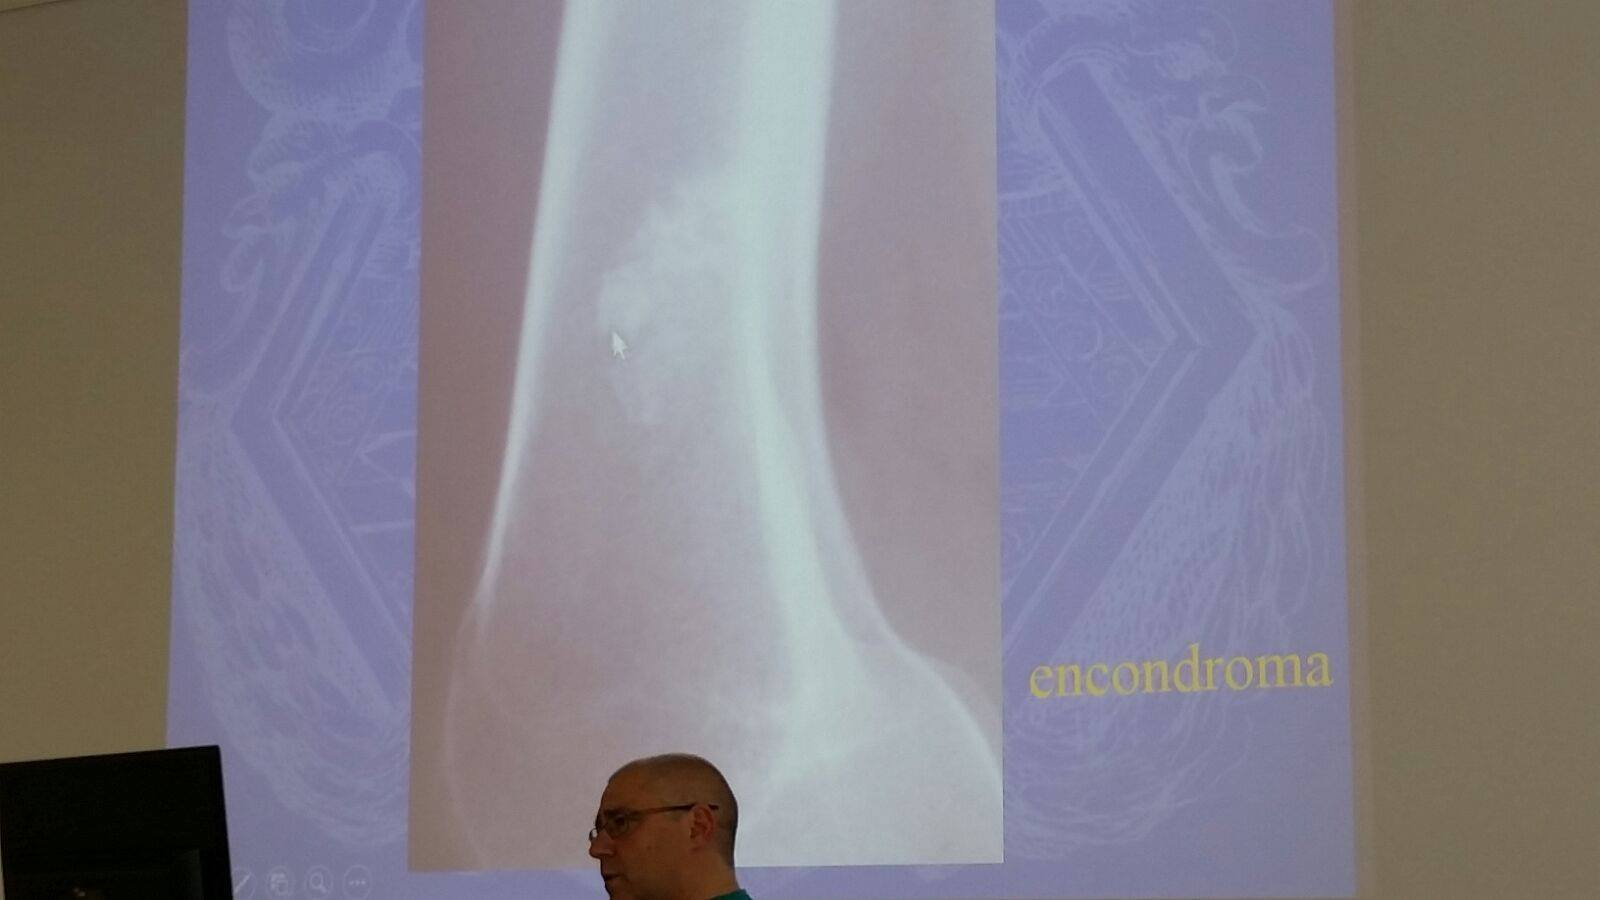
\includegraphics[width=4.17847in,height=3.22986in]{media/image1.jpeg}\textbf{recupero
  del tono-trofismo muscolare} (in quanto l'immobilizzazione prolungata
  determina una riduzione del tono muscolare)\textbf{.}
\end{itemize}

Generalmente una riabilitazione condotta in modo ottimale richiede
\textbf{3-4 settimane} (in quanto è necessario seguire gli ``step''
riportati sopra); a volte il \emph{dolore} è tale che impedisce di fare
tutto il resto ed è necessario prima di tutto tentare di
\emph{controllare il dolore stesso e la flogosi} (tp. farmacologica o
tp. strumentale) in questo modo una volta che riesco a far riassorbire
il versamento (dovuto alla flogosi) posso iniziare ad intervenire per
\emph{recuperare l'articolarità}. Infine intervengo per \emph{recuperare
e rinforzare il tono muscolare} che era diminuito a causa
dell'immobilizzazione.

Il \emph{tono muscolare} non è un fattore da trascurare e la
dimostrazione la si ha se si considera che i soggetti che svolgono
un'attività fisica importante, appena interrompono questa attività,
possono sviluppare una lombalgia (o una sintomatologia dolorosa lombare)
poiché perdono rapidamente il tono muscolare (è sufficiente un periodo
di stop di 5-7 giorni nei casi in cui si ha già una situazione di
compressione o sofferenza discale).

Cause di ipomobilità e dolore

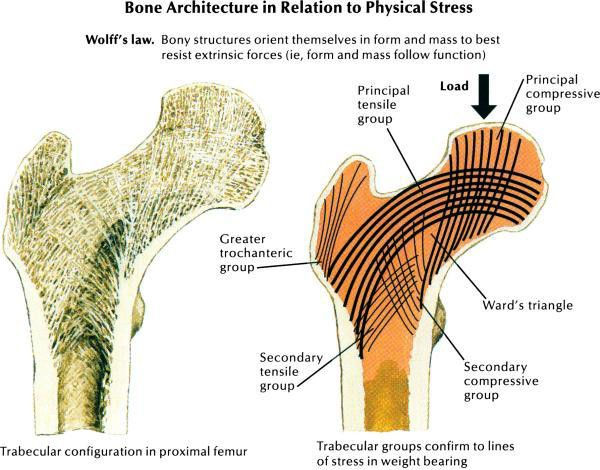
\includegraphics[width=4.43889in,height=3.43264in]{media/image2.jpeg}

Dopo un intervento chirurgico ci possono essere diverse
\textbf{situazioni che determinano dolore} \textbf{e che rallentano o
impediscono il processo di riabilitazione}.

La riabilitazione procede per step: si parla di ``flag'' (bandierine),
\emph{red flag} o \emph{yellow flag}, che indicano delle
``bandierine''-stop gialli o rossi a seconda che ci siano situazioni o
condizioni che non permettono di passare allo step riabilitativo
successivo. È quindi possibile passare allo step successivo solo se ci
sono condiziono adeguate.

Le \textbf{cause di ipomobilità e dolore} sono:

\begin{itemize}
\item
  fibrosi a livello dell'articolazione (\textbf{artrofibrosi})\textbf{;}
\end{itemize}

\begin{itemize}
\item
  \textbf{sindrome del ciclope} (condizione sovrapponibile
  all'artrofibrosi e che consiste nella \emph{formazione di tessuto
  fibroso all'interno dell'articolazione e più precisamente a livello
  della gola intercondiloidea} dove si innesta il legamento crociato;
  questo si verifica se il trattamento riabilitativo è particolarmente
  aggressivo, precoce, in condizioni non appropriate o, al contrario, se
  è ritardato)\textbf{;}
\item
  \textbf{sollecitazione inappropriata dell'innesto} (il LCA può essere
  sostituito con il tendine rotuleo, con il semitendinoso-gracile o con
  legamenti prelevati da cadavere o artificiali, di natura sintetica; i
  legamenti sintetici hanno il vantaggio di poter essere innestati in
  modo rapido e consentono un recupero molto veloce ma espongono a un
  maggior rischio di andare incontro ad artrosi);
\item
  \textbf{quadricipite - ischio-crurali ipostenici;}
\item
  \textbf{riabilitazione mal condotta;}
\item
  \textbf{immobilizzazione prolungata} (ad esempio in seguito ad un
  \emph{intervento chirurgico particolarmente aggressivo} o nel caso di
  un \emph{soggetto che presenta un'alterazione del processo di
  riparazione delle ferite;} ci sono ad esempio soggetti che vanno
  incontro a una cicatrizzazione eccesiva)\textbf{.}
\end{itemize}

Precocità dell'esercizio

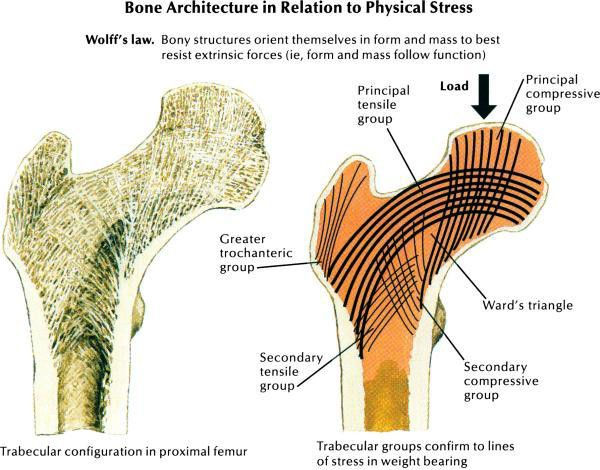
\includegraphics[width=4.59375in,height=3.55208in]{media/image3.jpeg}

Quando si parla di \emph{\textbf{esercizio precoce}} ci si riferisce ad
un \textbf{esercizio con \emph{carichi adeguati} in un \emph{arco di
movimento non doloroso }}(e solo in questo caso si può fare il discorso
dell'esercizio precoce perché, ad esempio, se i carichi non fossero
adeguati non otterremmo il risultato adeguato).

L'esercizio andrebbe cominciato quanto prima possibile.

L'\textbf{esercizio precoce} può portare a:

\begin{itemize}
\item
  una \textbf{migliore nutrizione della cartilagine;}
\item
  \textbf{riduzione dell'osteopenia da disuso/immobilizzazione;}
\item
  \textbf{riduzione della fibrosi perirotulea e del dolore;}
\item
  \textbf{più rapido ripristino della funzione del quadricipite} (il
  muscolo riesce ad ottenere un tono muscolare migliore).
\end{itemize}

Queste considerazioni si riferiscono al periodo \textbf{post-chirurgico}
ma, a maggior ragione, se nel periodo \textbf{pre-chirurgico} si
effettua un esercizio e si porta il soggetto in condizione fisica
adeguata il periodo post-chirurgico risulterà facilitato.

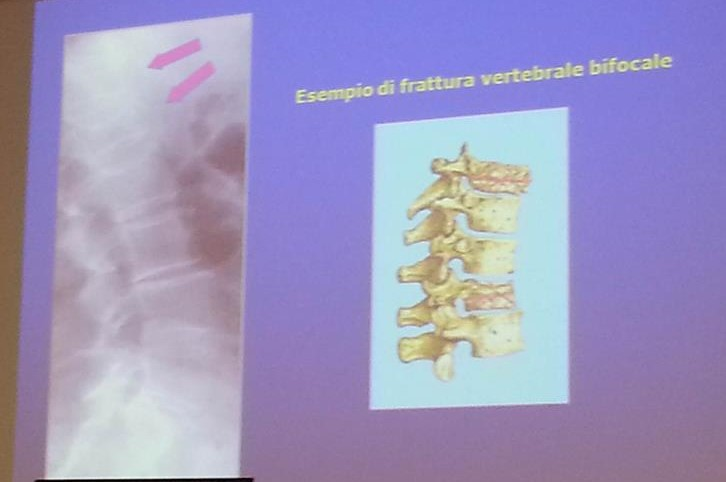
\includegraphics[width=5.04236in,height=3.89514in]{media/image4.jpeg}Gli
\textbf{esercizi precoci} andrebbero fatti in una condizione ben
definita che è la \textbf{catena cinetica chiusa.}

Esercizi in catena cinetica chiusa

Negli esercizi in catena cinetica chiusa \emph{l'articolazione} non
viene utilizzata in modo diretto ma \emph{viene utilizzata in modo tale
che sia inserita in un sistema che comprende altre articolazioni. }

L'articolazione del ginocchio, ad esempio, è situata tra l'articolazione
della caviglia e l'articolazione dell'anca.

In un esercizio di \emph{leg extension} (che simula un calcio) si
effettua un \textbf{esercizio in catena cinetica aperta} in quanto la
\emph{sollecitazione è solo sul ginocchio}.

Durante l'esecuzione di un esercizio su una \emph{pressa}, invece, si
effettua un esercizio in cui si spinge con i piedi e \emph{si utilizzano
diverse articolazioni} (tibio-tarsica, ginocchio, anca); in queste
condizioni \emph{il ginocchio è sollecitato meno} e riesce a sopportare
meglio le forze di taglio e angolari (di rotazione). (Esempio di un
\textbf{esercizio in catena cinetica chiusa.})

Durante l'esecuzione di esercizi in catena cinetica chiusa si ha:

\begin{itemize}
\item
  \textbf{co-contrazione di quadricipite e ischio-crurali} con:
\end{itemize}

\begin{enumerate}
\def\labelenumi{\arabic{enumi}.}
\item
  \emph{protezione del legamento crociato anteriore,}

  \emph{riduzione delle forze di taglio anteriori che agiscono
  sull'innesto.}
\end{enumerate}

\begin{quote}
Le articolazioni sono costituite da 3 componenti: componente ossea,
componente legamentosa e componente muscolare; osso e legamenti
rappresentano le componenti statiche, i muscoli rappresentano le
componenti dinamiche. Se si effettua un movimento in cui il ginocchio
non viene sollecitato direttamente si preserva l'innesto del legamento
crociato anteriore e si evitano i movimenti di traslazione anteriore
\emph{(movimenti del cassetto; i movimenti del cassetto sono una manovra
semiologia che, durante l'esame obiettivo, consentono di valutare la
lesione del legamento crociato anteriore (test del cassetto anteriore) o
del legamento crociato posteriore (test del cassetto posteriore); un
altro test che si può fare per valutare le lesioni del crociato
anteriore è il test di lachman, simile a quello del cassetto).}
\end{quote}

\begin{enumerate}
\def\labelenumi{\arabic{enumi}.}
\item
  \textbf{minor traslazione anteriore della tibia} (vedi
  sopra)\textbf{;}

  \textbf{rinforzo dei muscoli Vasti (rispetto al muscolo retto
  femorale).} Il muscolo quadricipite è un muscolo costituito da diverse
  componenti (retto femorale, vasto mediale, vasto laterale). I muscoli
  vasto mediale e vasto laterale hanno un effetto molto importante sulla
  rotula. La \emph{rotula} è messa in una posizione tale che
  \emph{aumenta il braccio di leva del muscolo quadricipite}: il
  quadricipite, grazie alla rotula, riesce ad esprimere un forza
  maggiore rispetto a quella che avrebbe se si inserisse direttamente su
  un'articolazione perché la rotula è mobile e garantisce un'inserzione
  più bassa (il quadricipite si inserisce sulla rotula e questa si
  inserisce più in basso, sul tubercolo). La rotula, per poter esprimere
  la massima forza, deve muoversi in modo preciso. Sulla superficie
  inferiore, articolare, della rotula è presente una cresta che consente
  un movimento obbligato di questo osso all'interno di una gola. Se la
  rotula non si muove perfettamente in questa gola si crea attrito e si
  possono avere lesioni cartilaginee (con condropatie e dolore che
  possono compromettere il trattamento riabilitativo del ginocchio).
  Vasto laterale e vasto mediale devono lavorare in maniera ottimale in
  modo tale che si contragga \emph{prima} l'uno (\emph{vasto mediale}) e
  \emph{poi} l'altro (\emph{vasto laterale}), questo perché quando la
  rotula scivola tende a lateralizzarsi, tende ad andare verso l'esterno
  (inoltre, quando si ha una lussazione della rotula nel 90\% dei casi
  la lussazione è laterale); \emph{la contrazione dei muscoli vasti deve
  avvenire con un timing adeguato in modo tale che si attivi
  \textbf{prima il muscolo vasto mediale, poi il muscolo vasto
  laterale.}} A volte il segnale di attivazione non arriva in maniera
  adeguata e si attiva prima il vasto laterale e poi il vasto mediale,
  la rotula inizia a spostarsi verso l'esterno e se il vasto mediale non
  è sufficientemente forte per riportare la rotula in sede centrale si
  creano attriti; ciò può causare dolore e infiammazioni (come
  l'infiammazione del batuffolo di Hoffa, localizzato sopra il
  ginocchio, o l'infiammazione del tendine rotuleo).
\end{enumerate}

\textbf{Test del cassetto (anteriore)}. Viene effettuato con il paziente
a ginocchio flesso a 90°. L'operatore posiziona una mano dietro al
ginocchio ed effettua un movimento di traslazione anteriore. Se la tibia
trasla in avanti rispetto al femore è segno di lesione del crociato; a
seconda dell'entità dello spostamento della tibia la lesione potrà
essere parziale o totale.

Attenzione a soggetti che possono presentare una lassità costituzionale
della capsula e dei legamenti per cui si può pensare che il test del
cassetto sia positivo quando in realtà non si ha lesione dei legamenti.
È sempre importante fare una \emph{valutazione comparativa} di entrambe
le articolazioni (quella di destra e quella di sinistra) assicurandosi
che il soggetto non abbia subito altri traumi distorsivi all'altro
ginocchio. Un altro aspetto importante da tenere in considerazione è che
chi ha una lassità legamentosa a livello del ginocchio avrà anche una
lassità legamentosa a livello delle caviglie e dei polsi (valutare anche
la mobilità di queste articolazioni).

\textbf{Test di Lachman}. Il principio di base è lo stesso del test del
cassetto ma in questo caso il ginocchio è esteso. (Una mano è sul femore
e lo tiene fermo, l'altra mano trazione la tibia; si valutano eventuali
movimenti di traslazione.)

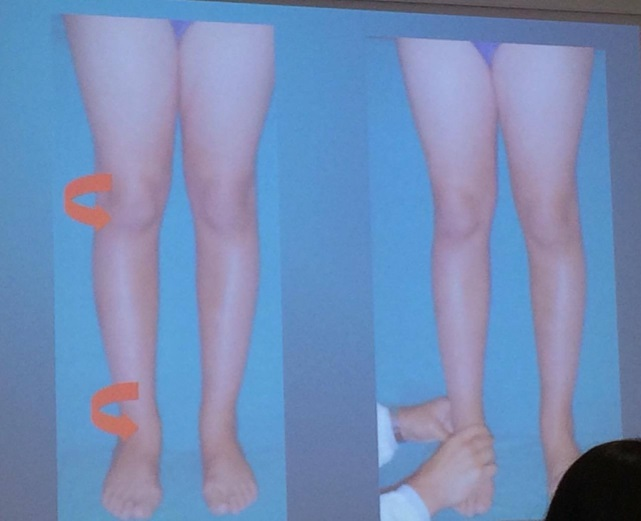
\includegraphics[width=4.05556in,height=3.13403in]{media/image5.jpeg}Valutazione
posturale

In un soggetto che abbia subito un intervento di ricostruzione del LCA è
necessario fare una \emph{valutazione posturale frontale, laterale e
posteriore} per vedere se ci sono asimmetrie o altre condizioni
particolari.

Se poi si vuole fare una valutazione più accurata si può effettuare una
\textbf{stabilometria} che permette di rilevare le oscillazioni del
soggetto.

Stabilometria

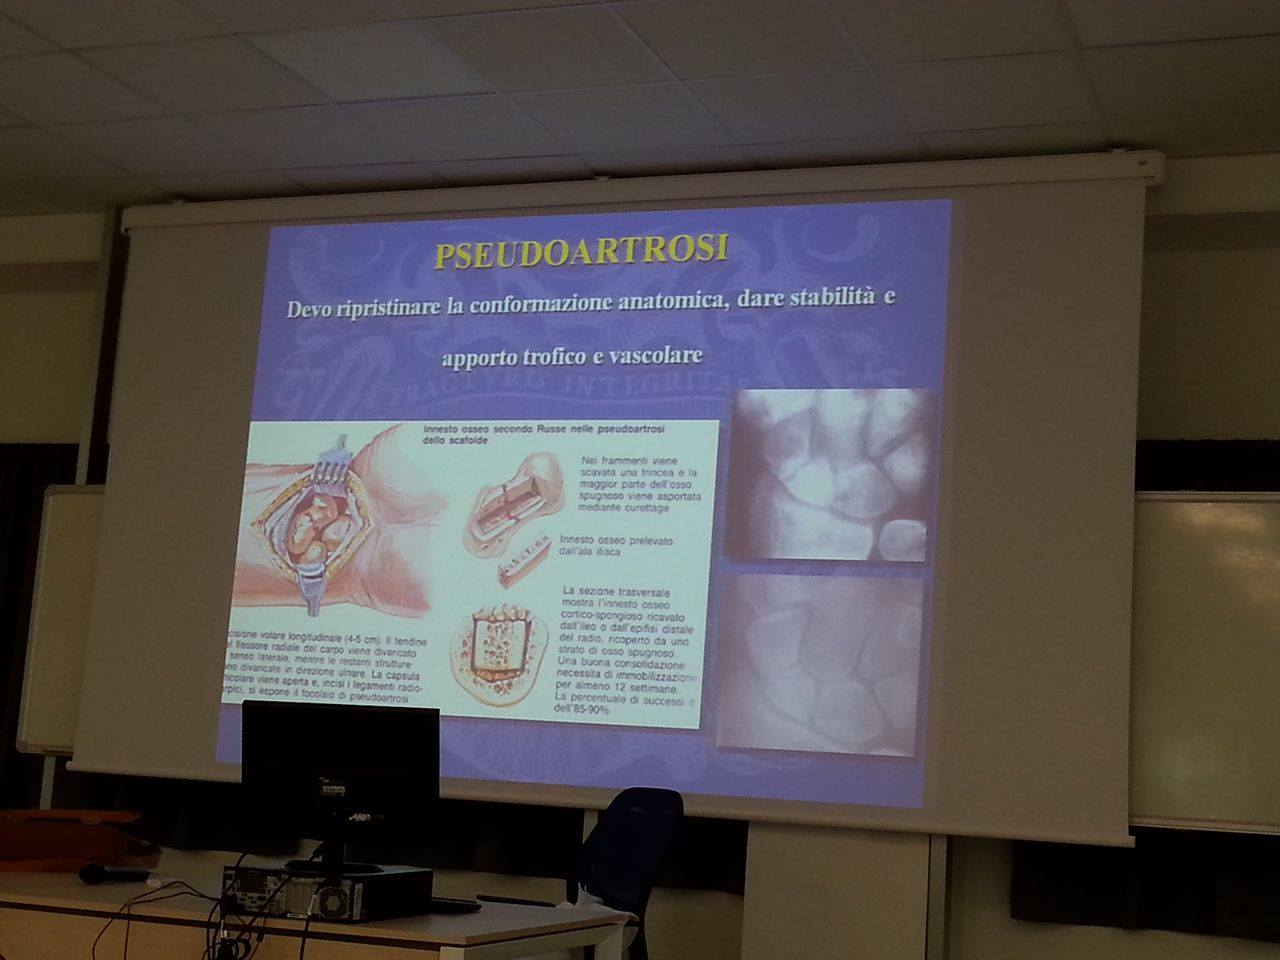
\includegraphics[width=3.35764in,height=2.38125in]{media/image6.jpeg}

Con la stabilometria è possibile registrare le oscillazioni del
soggetto.

(Nella diapositiva è possibile vedere come le oscillazioni prima
dell'intervento siano molto più ampie rispetto a quelle registrate dopo
l'intervento e trattamento riabilitativo: questo sta ad indicare che il
soggetto riesce a percepire meglio la sua posizione i movimenti che fa.)

\emph{Generalmente dopo l'intervento e il trattamento riabilitativo il
soggetto riesce a percepire meglio la sua posizione e i movimenti che fa
e le oscillazioni registrate mediante stabilometria risultano molto più
contenute rispetto a quelle che vengono registrate prima
dell'intervento. }

Rieducazione propriocettiva

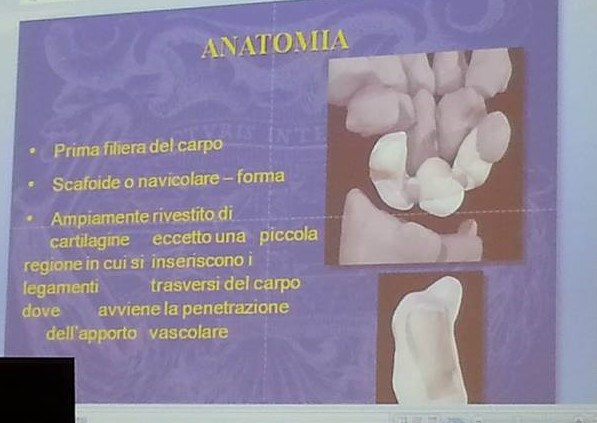
\includegraphics[width=4.05903in,height=3.13750in]{media/image7.jpeg}

La rieducazione propriocettiva è molto importante in quanto dobbiamo
fare in modo che il nostro soggetto abbia la consapevolezza e la
coscienza dei movimenti che è in grado di fare e degli stimoli che
partono dal ginocchio. (In realtà ci sono stimoli ascendenti,
dall'appoggio, e stimoli discendenti, per stimolazione diretta dei
recettori del ginocchio che portano impulsi a livello centrale si ha una
risposta riflessa per cui si attivano i muscoli del ginocchio).

Il LCA integro contiene propriocettori (corpuscoli del Pacini,
corpuscoli del Ruffini e terminazioni nervose libere).

Questi propriocettori possono essere stimolati tramite
\textbf{tavolette} di varie forme e dimensioni con vari assi di
movimento. Il soggetto sale al di sopra di queste tavolette e può
eseguire esercizi sempre più complessi e destabilizzanti; il grado di
destabilizzazione può essere aumentato mettendo in difficoltà il
soggetto: si fa eseguire l'esercizio prima in carico bipodalico e poi in
carico monopodalico; posso anche far compiere al soggetto dei compiti
diversi (faccio mettere il soggetto su un piede su una pedana tonda, che
risulta più complessa di una pedana rettangolare, e posso lanciargli una
pallina che deve afferrare; se il soggetto gioca a pallavolo posso
chiedergli di eseguire palleggi o bagher ecc\ldots{}). Se voglio
destabilizzare il soggetto ancora di più posso deprivarlo della visione.

In centri attrezzati sono disponibili \textbf{pedane vibratorie}. La
pedana vibratoria trasmette una vibrazione al piede che va a stimolare
recettori propriocettivi. È possibile assumere diverse posizioni sulla
pedana in modo da variare la stimolazione vibratoria nella zona
desiderata e
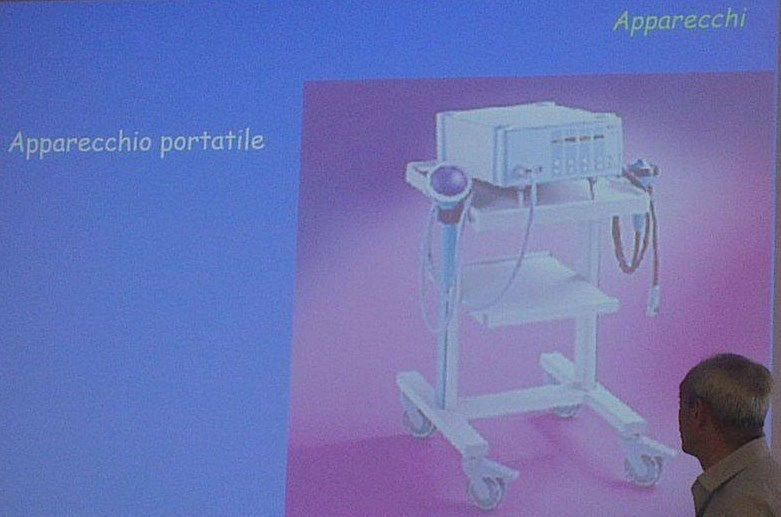
\includegraphics[width=3.26806in,height=2.52708in]{media/image8.jpeg}inoltre
pedane diverse possono vibrare a frequenze diverse.

Pedana vibratoria

Nei protocolli più seguiti vengono utilizzate pedane che vibrano a una
\textbf{frequenza di 25 Hz}.

Si effettua \textbf{1 serie da 6 ripetizioni con una pausa di 1 minuto}.

È molto importante anche il modo in cui viene effettuata questa attività
soprattutto in relazione all'\emph{angolo} che si crea quando il
soggetto flette il ginocchio:

\begin{enumerate}
\def\labelenumi{\arabic{enumi}.}
\item
  se il soggetto sta in piedi e non flette il ginocchio la vibrazione si
  trasmette anche a strutture al di sopra del ginocchio;

  se invece il soggetto flette il ginocchio la vibrazione agisce
  principalmente su questa articolazione.
\end{enumerate}

\emph{Più il soggetto flette il ginocchio (e chiude l'angolo) più
l'articolazione è sottoposta all'azione della vibrazione. }

Se un soggetto sale su una pedana vibratoria ferma e si mette in
flessione e misura la sua altezza dal terreno, dopo 1 minuto di
applicazione di vibrazione, se questo soggetto si rimette in flessione e
valuta la sua altezza da terra noterà che sarà diminuita in quanto
\emph{lo stimolo propriocettivo dato dalla vibrazione ha un effetto di
rilassamento sulla muscolatura.}

Il rilassamento della muscolatura garantisce una miglior azione
muscolare soprattutto per quanto riguarda il muscolo antagonista il
quale deve controllare che l'effetto del muscolo agonista, che determina
il movimento, sia adeguato.

Vantaggi della piattaforma vibratoria

Tonificazione senza sovraccarico alle articolazioni

Aumento della forza

Rilassamento dei muscoli antagonisti

Diminuzione del dispendio energetico e dell'affaticamento

Coordinazione neuromuscolare (prevenzione infortuni)

Qualità della risposta motoria e miglior risposta posturale

Aumenta il tono calcico nella prevenzione dell'osteoporosi

E' di aiuto nella prevenzione della lombalgia su base muscolotensiva

Recupero accellerato nel Post-Operatorio di ricostruzioni di LCA 135

Riscontrati risultati di alto livello nelle prestazioni degli atleti
professionisti

Controindicazioni

• Patologia acuta

• Retinopatie

• Patologie neuromotorie (sclerosi multipla, Parkinson)

• Sciatalgie, compressioni radici nervose

• Epilessia

• Portatori pace-maker

• Gravidanza

• Portatrici di spirale

• Assunzione costante di cortisone

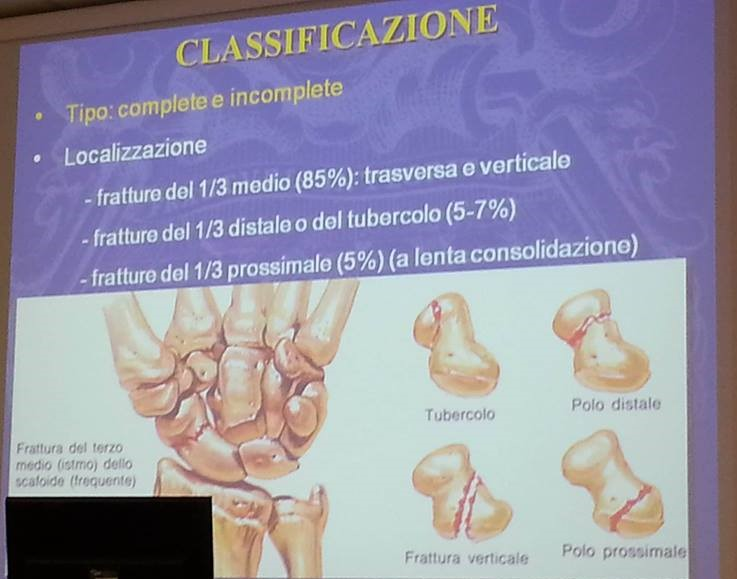
\includegraphics[width=4.52222in,height=3.49375in]{media/image9.jpeg}Muscle
LAB

\textbf{Dinamometro Isotonico.} Strumento utilizzato in passato. Il
dinamometro è dotato di un sensore (\emph{encoder}, indicato nella
figura) che viene applicato a macchine da muscolazione in palestra.

Il dispositivo è in grado di individuare una \emph{curva forza-velocità}
tramite la quale è possibile risalire alla forza del soggetto.

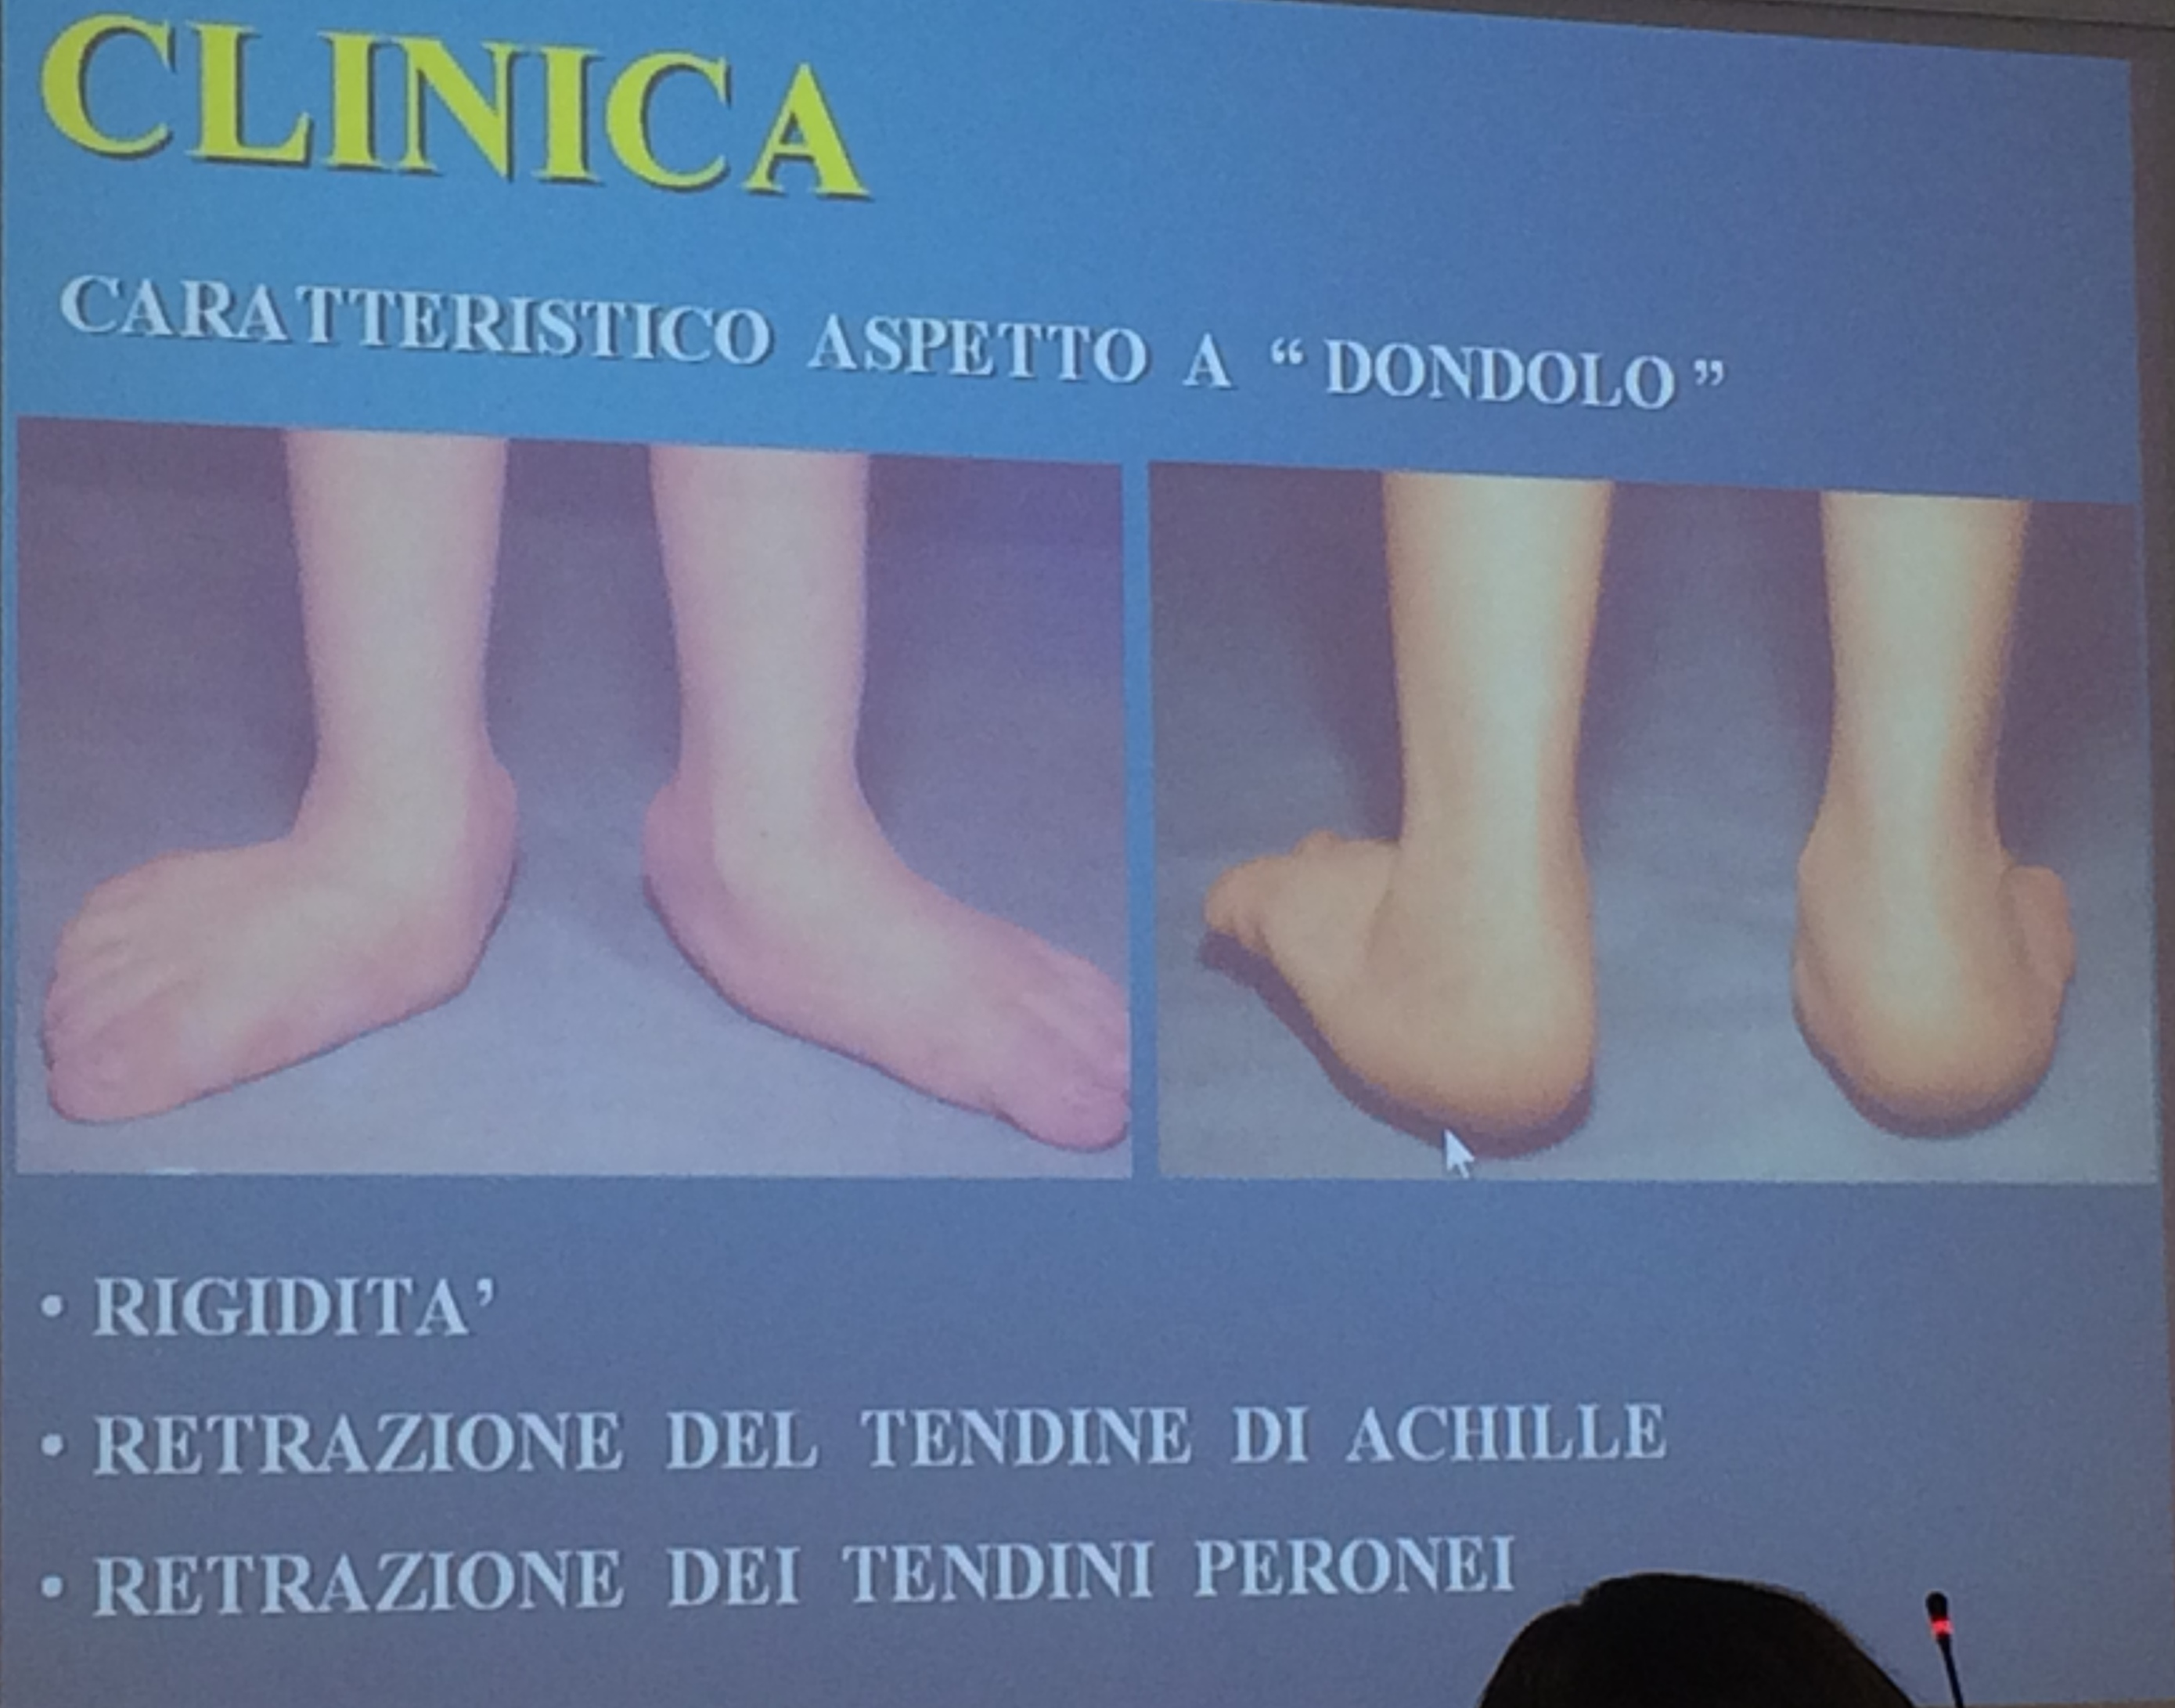
\includegraphics[width=5.84583in,height=4.14861in]{media/image10.jpeg}

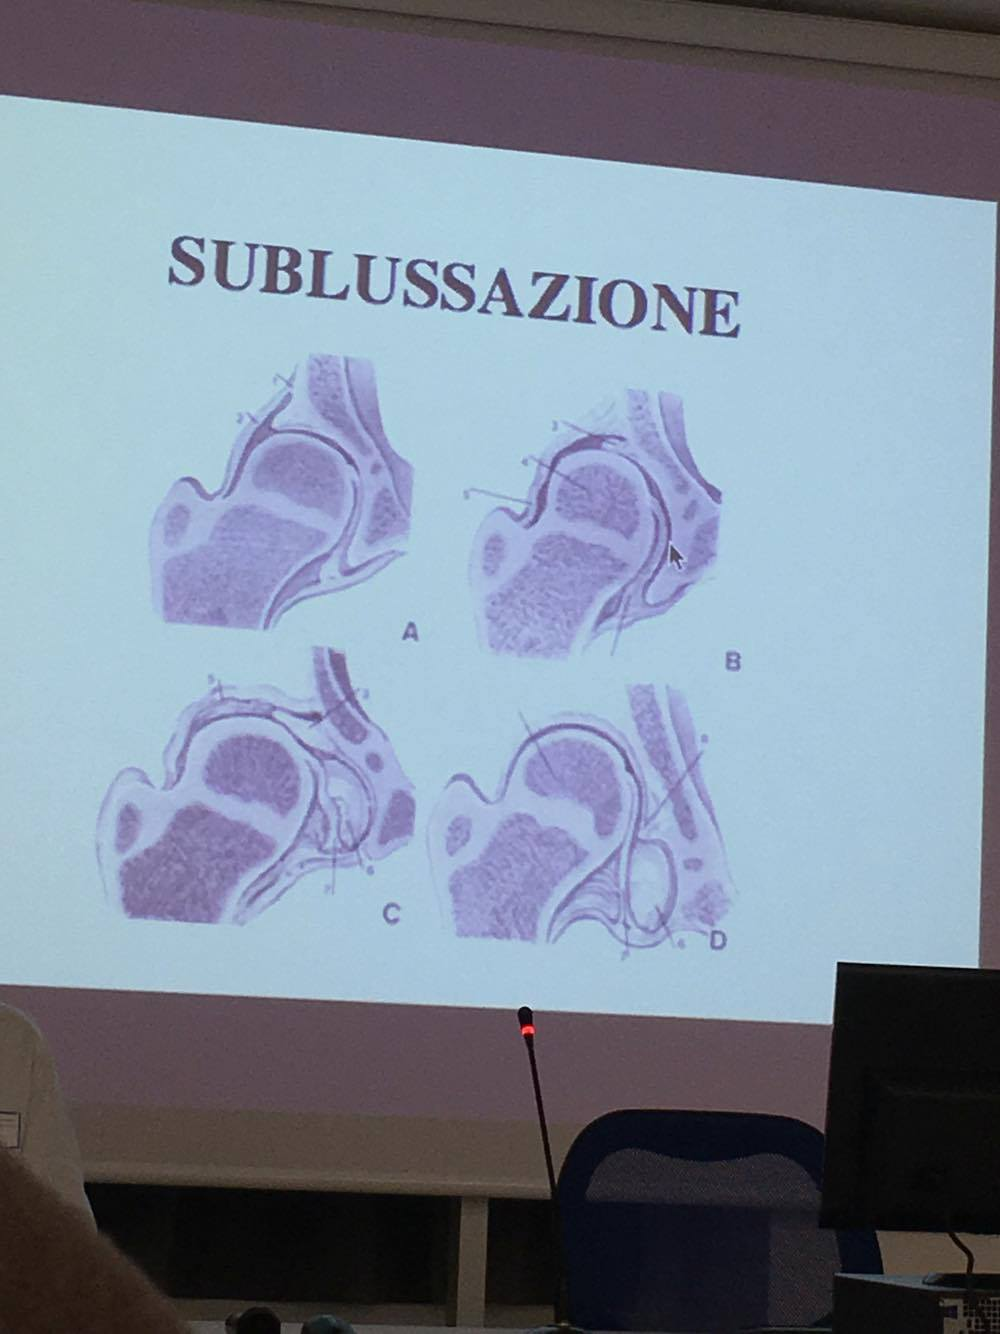
\includegraphics[width=7.14879in,height=5.52239in]{media/image11.jpeg}Elettromiografia
superficiale

L'\textbf{elettromiografia superficiale} può fornire informazioni
importanti.

È possibile ricavare il \emph{rapporto tra muscoli agonisti e muscoli
antagonisti} prima e dopo il trattamento.

Ci sono anche elettrodi particolari che consentono di valutare come
avviene la contrazione muscolare del soggetto (ad esempio se sta
avvenendo in maniera adeguata).

Pedana di forza

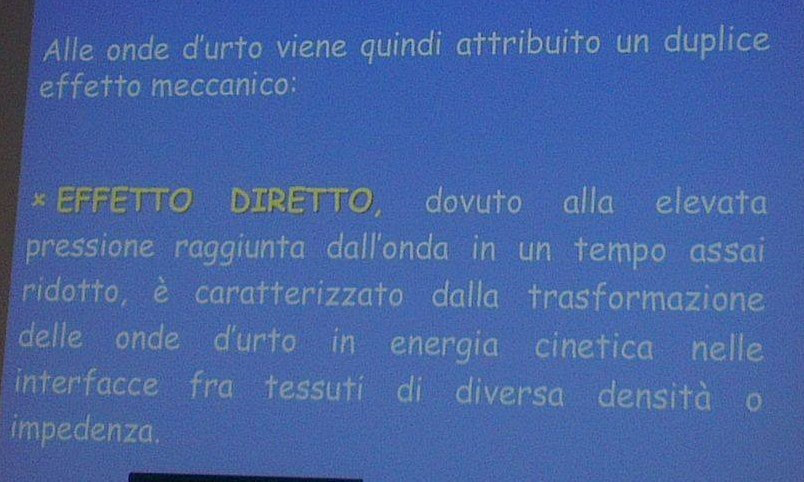
\includegraphics[width=5.11181in,height=3.62639in]{media/image12.jpeg}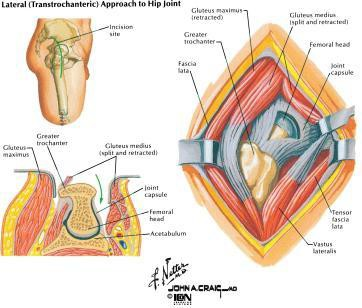
\includegraphics[width=3.99167in,height=3.08542in]{media/image13.jpeg}È
possibile effettuare dei \emph{test di forza} per valutare la
\emph{forza esplosiva. }

Quando si va a rinforzare un muscolo si può agire in modi diversi per
sviluppare un particolare tipo di forza rispetto a un altro.

La \textbf{forza} può essere:

\begin{enumerate}
\def\labelenumi{\arabic{enumi}.}
\item
  \textbf{esplosiva},

  \textbf{resistente},

  \textbf{stiffness} (capacità di mantenere un'attività muscolare
  continua a livello di un'articolazione).
\end{enumerate}

La \textbf{pedana di forza} mi permette di effettuare un test per
valutare la forza muscolare.

Isocinetica

L'\textbf{isocinetica} è un'altra possibilita che ci consente di fare
una valutazione dei muscoli e permette una sovrapposizione delle
valutazioni per fare confronti (ad esempio, valuto il quadricipite e gli
ischio-crurali e posso poi fare dei confronti).

È anche possibile fare una elettromiografia per vedere come si attivano
e come lavorano i muscoli. Dal tracciato è possibile individuare il
momento in cui il muscolo raggiunge l'affaticamento (si avrà un
tracciato ``a rombo'' e molto più ampio rispetto al tracciato che si ha
all'inizio dell'attività muscolare). Una volta che il muscolo si è
affaticato l'ulteriore lavoro
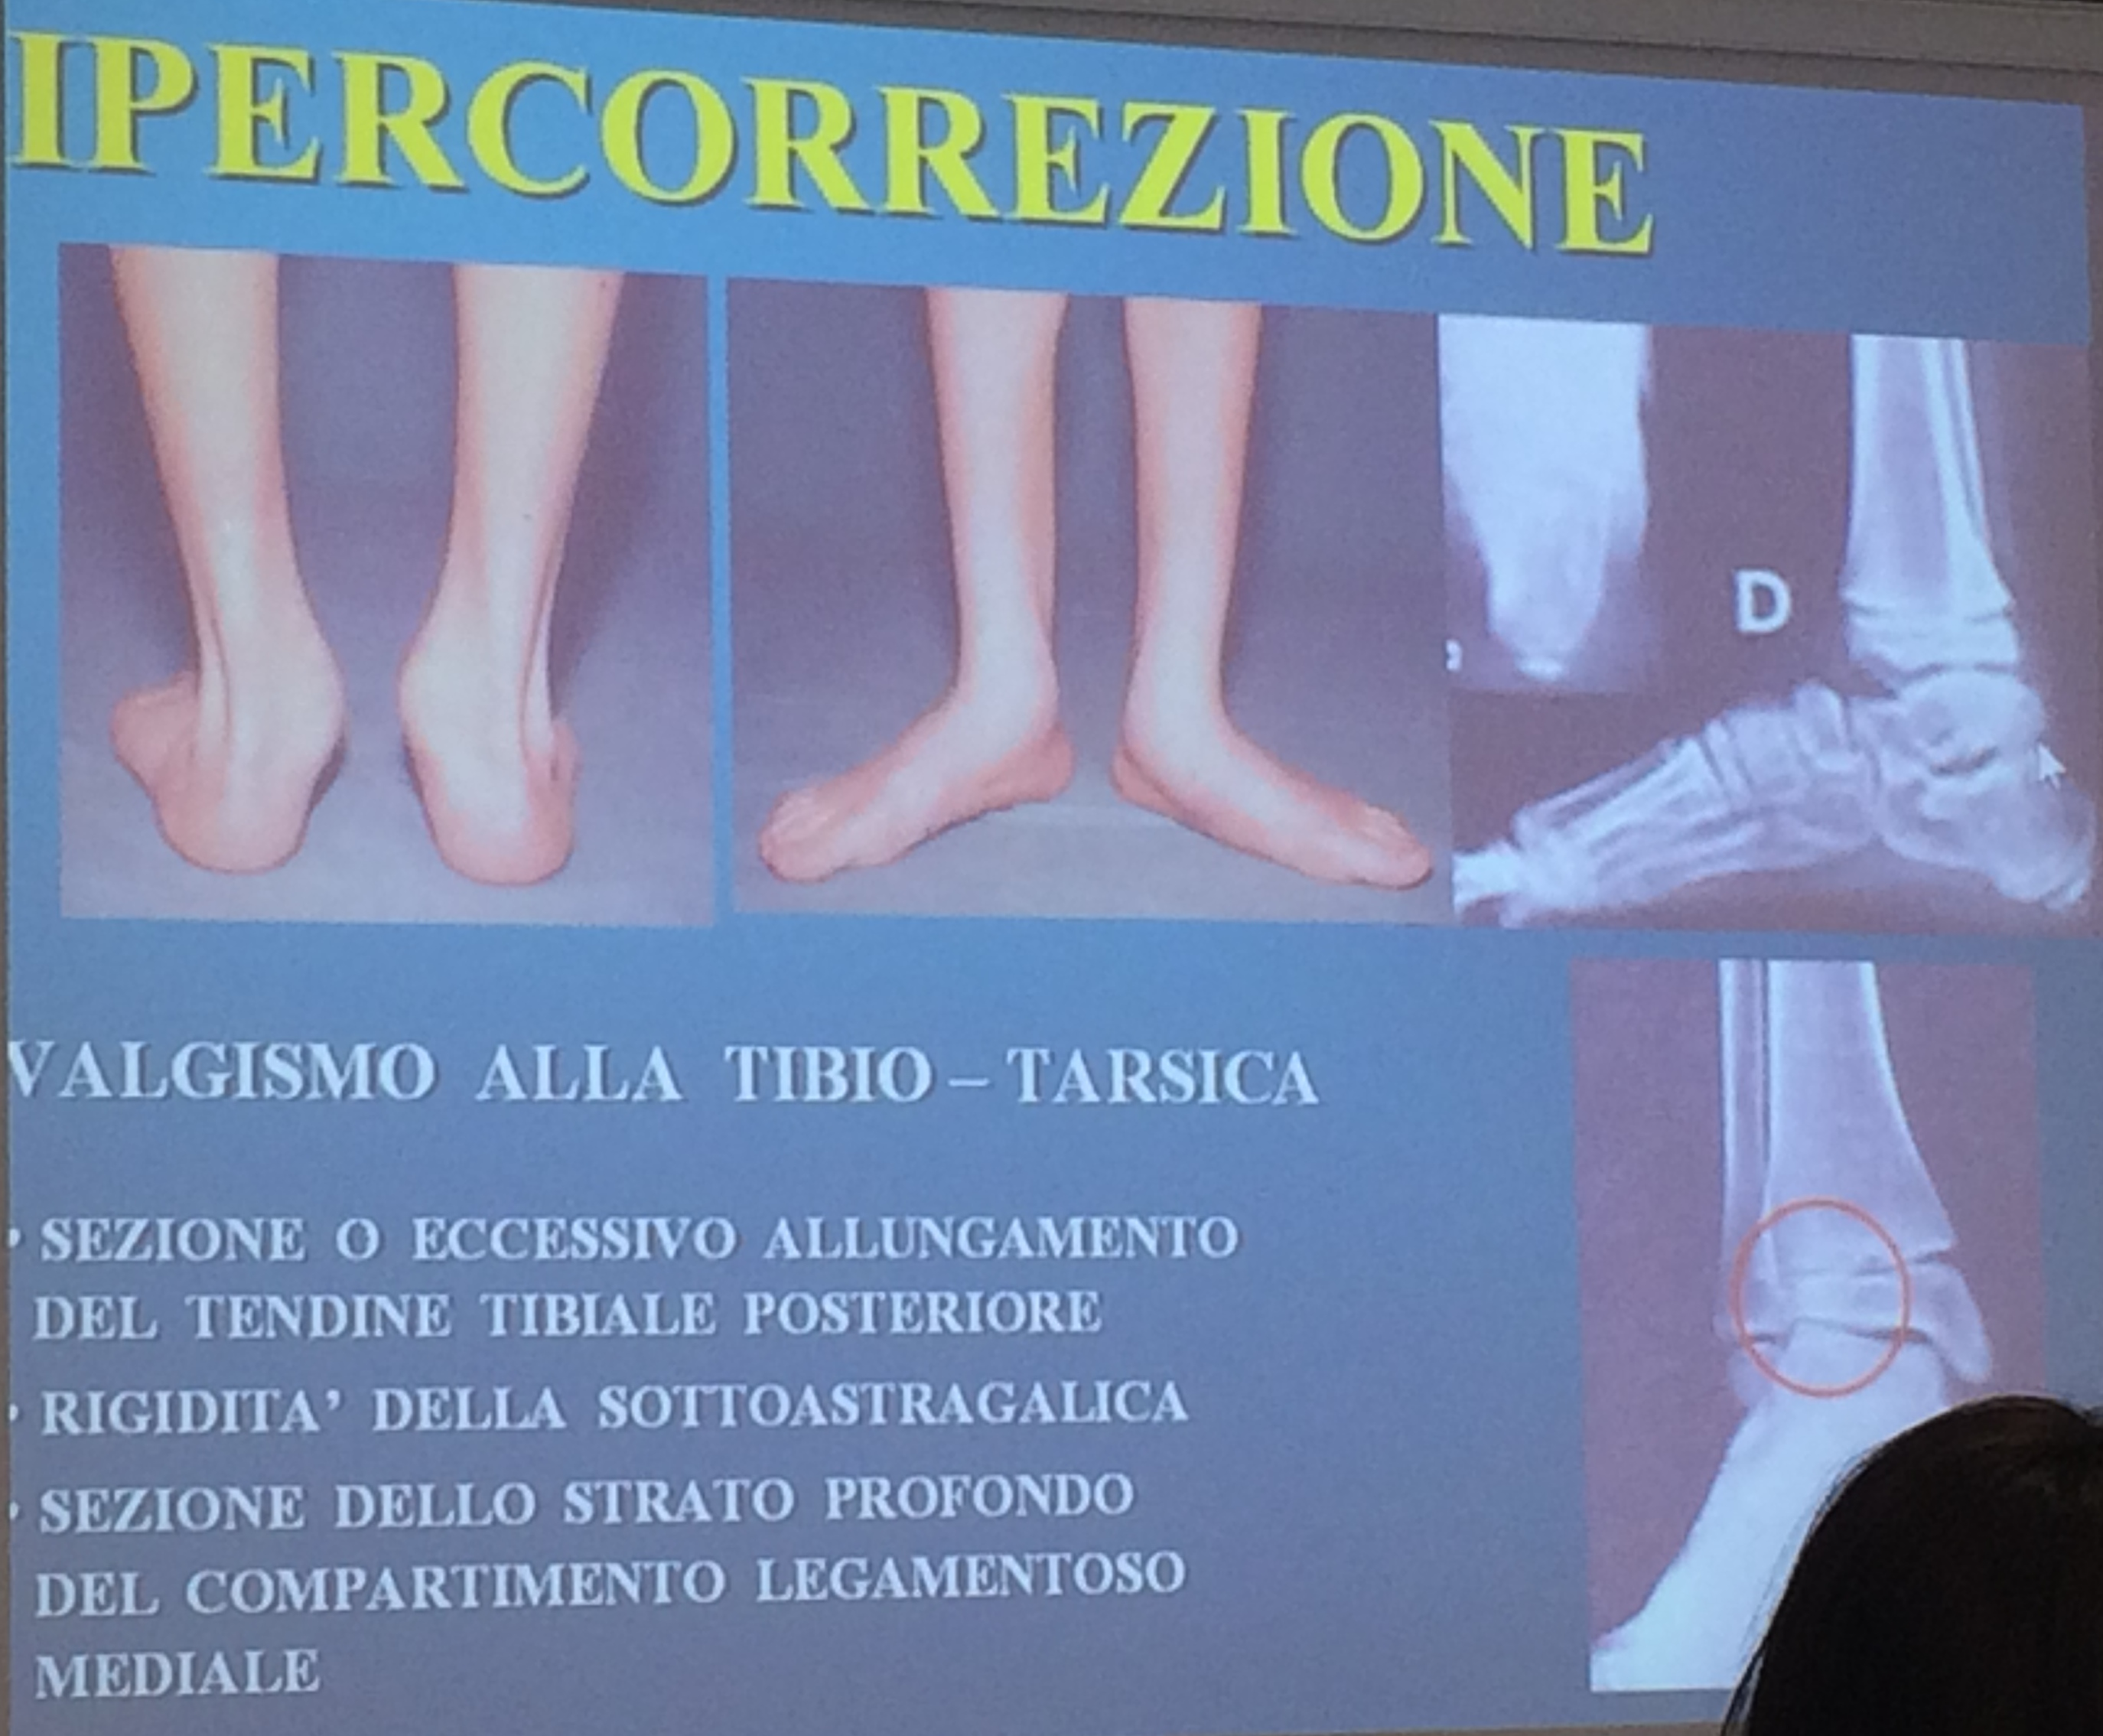
\includegraphics[width=6.04413in,height=4.67164in]{media/image14.jpeg}muscolare
ha conseguenze negative sul muscolo stesso.

Gayt Analysis e Baropodometria Dinamica

La \textbf{Gayt Analysis} è l'\emph{analisi del movimento} e può essere
fatta con diversi sistemi, ad esempio:

\begin{enumerate}
\def\labelenumi{\arabic{enumi}.}
\item
  sistemi che analizzano il movimento in modo cinematografico tramite
  telecamere posizionate posteriormente al soggetto;
\end{enumerate}

\begin{enumerate}
\def\labelenumi{\arabic{enumi}.}
\item
  \emph{sistemi optoelettronici} con 6-8 telecamere che consentono di
  vedere tutti i movimenti.
\end{enumerate}

La \textbf{baropodometria} permette di misurare \emph{quanto appoggia,
come appoggia e come distribuisce il carico il soggetto} (riesco a
vedere in che modo viene distribuita la pressione esercitata dal piede
destro e dal piede sinistro).

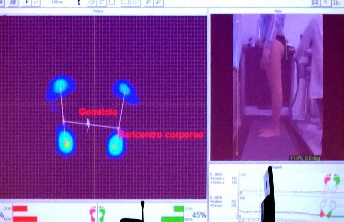
\includegraphics[width=5.03264in,height=3.25556in]{media/image15.jpeg}Fornisce
informazioni anche sul \emph{baricentro} del soggetto e su come si
posiziona (la rieducazione postulare globale ha proprio la funzione di
rimettere in asse il soggetto).

Tramite queste metodiche possiamo valutare il soggetto durante
l'attività (quando è in movimento) e possiamo fare un'\emph{analisi del
passo} (attraverso un'analisi dei singoli appoggi e dello
stabilogramma).

Taping neuromuscolare

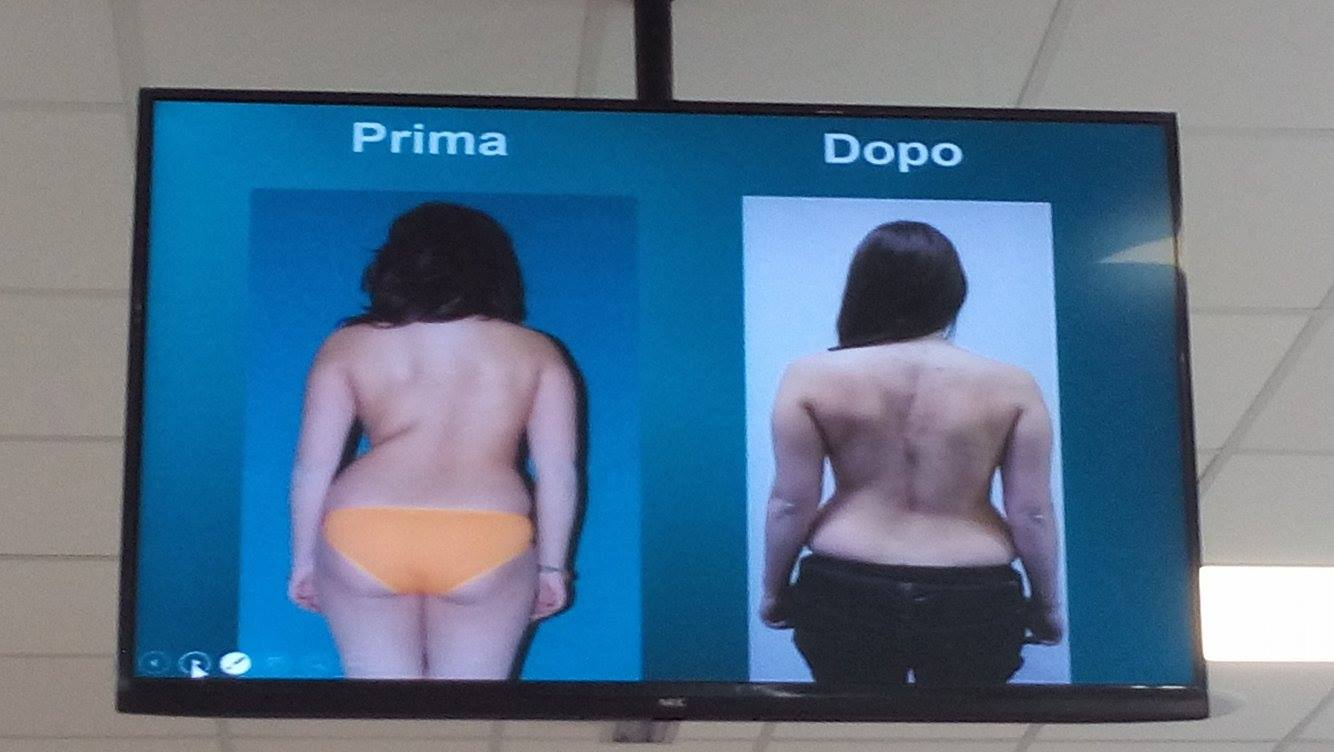
\includegraphics[width=3.40278in,height=2.62986in]{media/image16.jpeg}

Il \textbf{taping neuromuscolare} consiste nell'applicare delle fasce
adesive sulla cute che esercitano uno \emph{stimolo propriocettivo}.

È stato fatto uno studio in cui un gruppo di soggetti faceva un
trattamento riabilitativo normale mentre un altro gruppo faceva il
trattamento normale e in più metteva il tape. Ciò che è emerso da questo
studio è stato che i soggetti del secondo gruppo, quelli che erano stati
trattato con il \emph{taping}, mostravano un miglioramento della forza
muscolare del 7-9\%. Questo miglioramento ha poi delle ripercussioni
anche sui tempi di recupero (che risultano ridotti).

Lo stesso studio è stato fatto anche per quanto riguarda la \emph{pedana
vibratoria} e anche in questo caso è stato visto che i soggetti trattati
con pedana vibratoria mostravano dei buoni risultati.

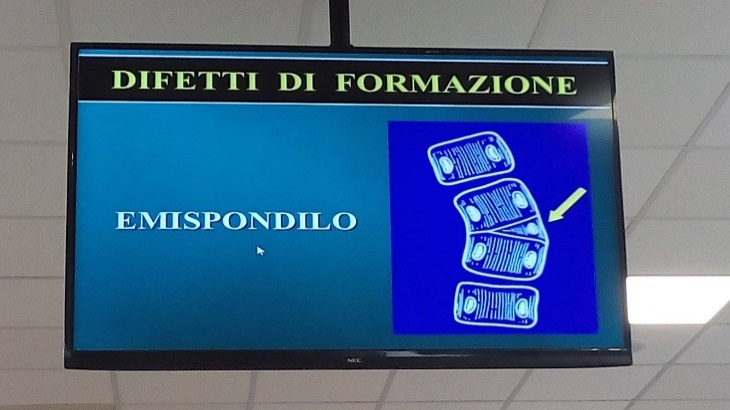
\includegraphics[width=4.29792in,height=3.32222in]{media/image17.jpeg}

Le fasce adesive possono essere applicate in modo diverso e in sedi
diverse. Esempi:

\begin{enumerate}
\def\labelenumi{\arabic{enumi}.}
\item
  è possibile \emph{applicare le fasce sugli ischio-crurali} in modo
  tale da creare una stimolazione simile a un micro-massaggio che
  \emph{riduce la tensione muscolare}; la tensione di questi muscoli
  determina un sovraccarico della rotula ed è quindi importante cercare
  di ridurla;

  le fasce possono essere \emph{applicate sulla rotula} per creare un
  \emph{effetto di liberazione della rotula} stessa e per \emph{ridurre
  la tendenza della rotula a lateralizzarsi};

  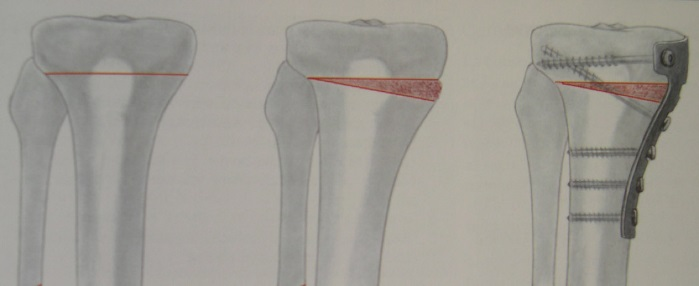
\includegraphics[width=3.85959in,height=2.98349in]{media/image18.jpeg}applicate
  sulle articolazioni possono favorire il \emph{drenaggio di eventuali
  versamenti};

  in caso di \emph{tendinite rotulea} queste fasce possono garantire una
  \emph{stabilizzazione sottorotulea.}
\end{enumerate}

Il taping neuromuscolare può essere utilizzato anche sulle macchine per
consentire al soggetto di esprimere forza maggiore.

La vibrazione applicata direttamente su un muscolo fa in modo che la
percezione di quel muscolo sia diversa.

È stato fatto un esperimento sugli sportivi. Viene preso in
considerazione il bicipite brachiale
e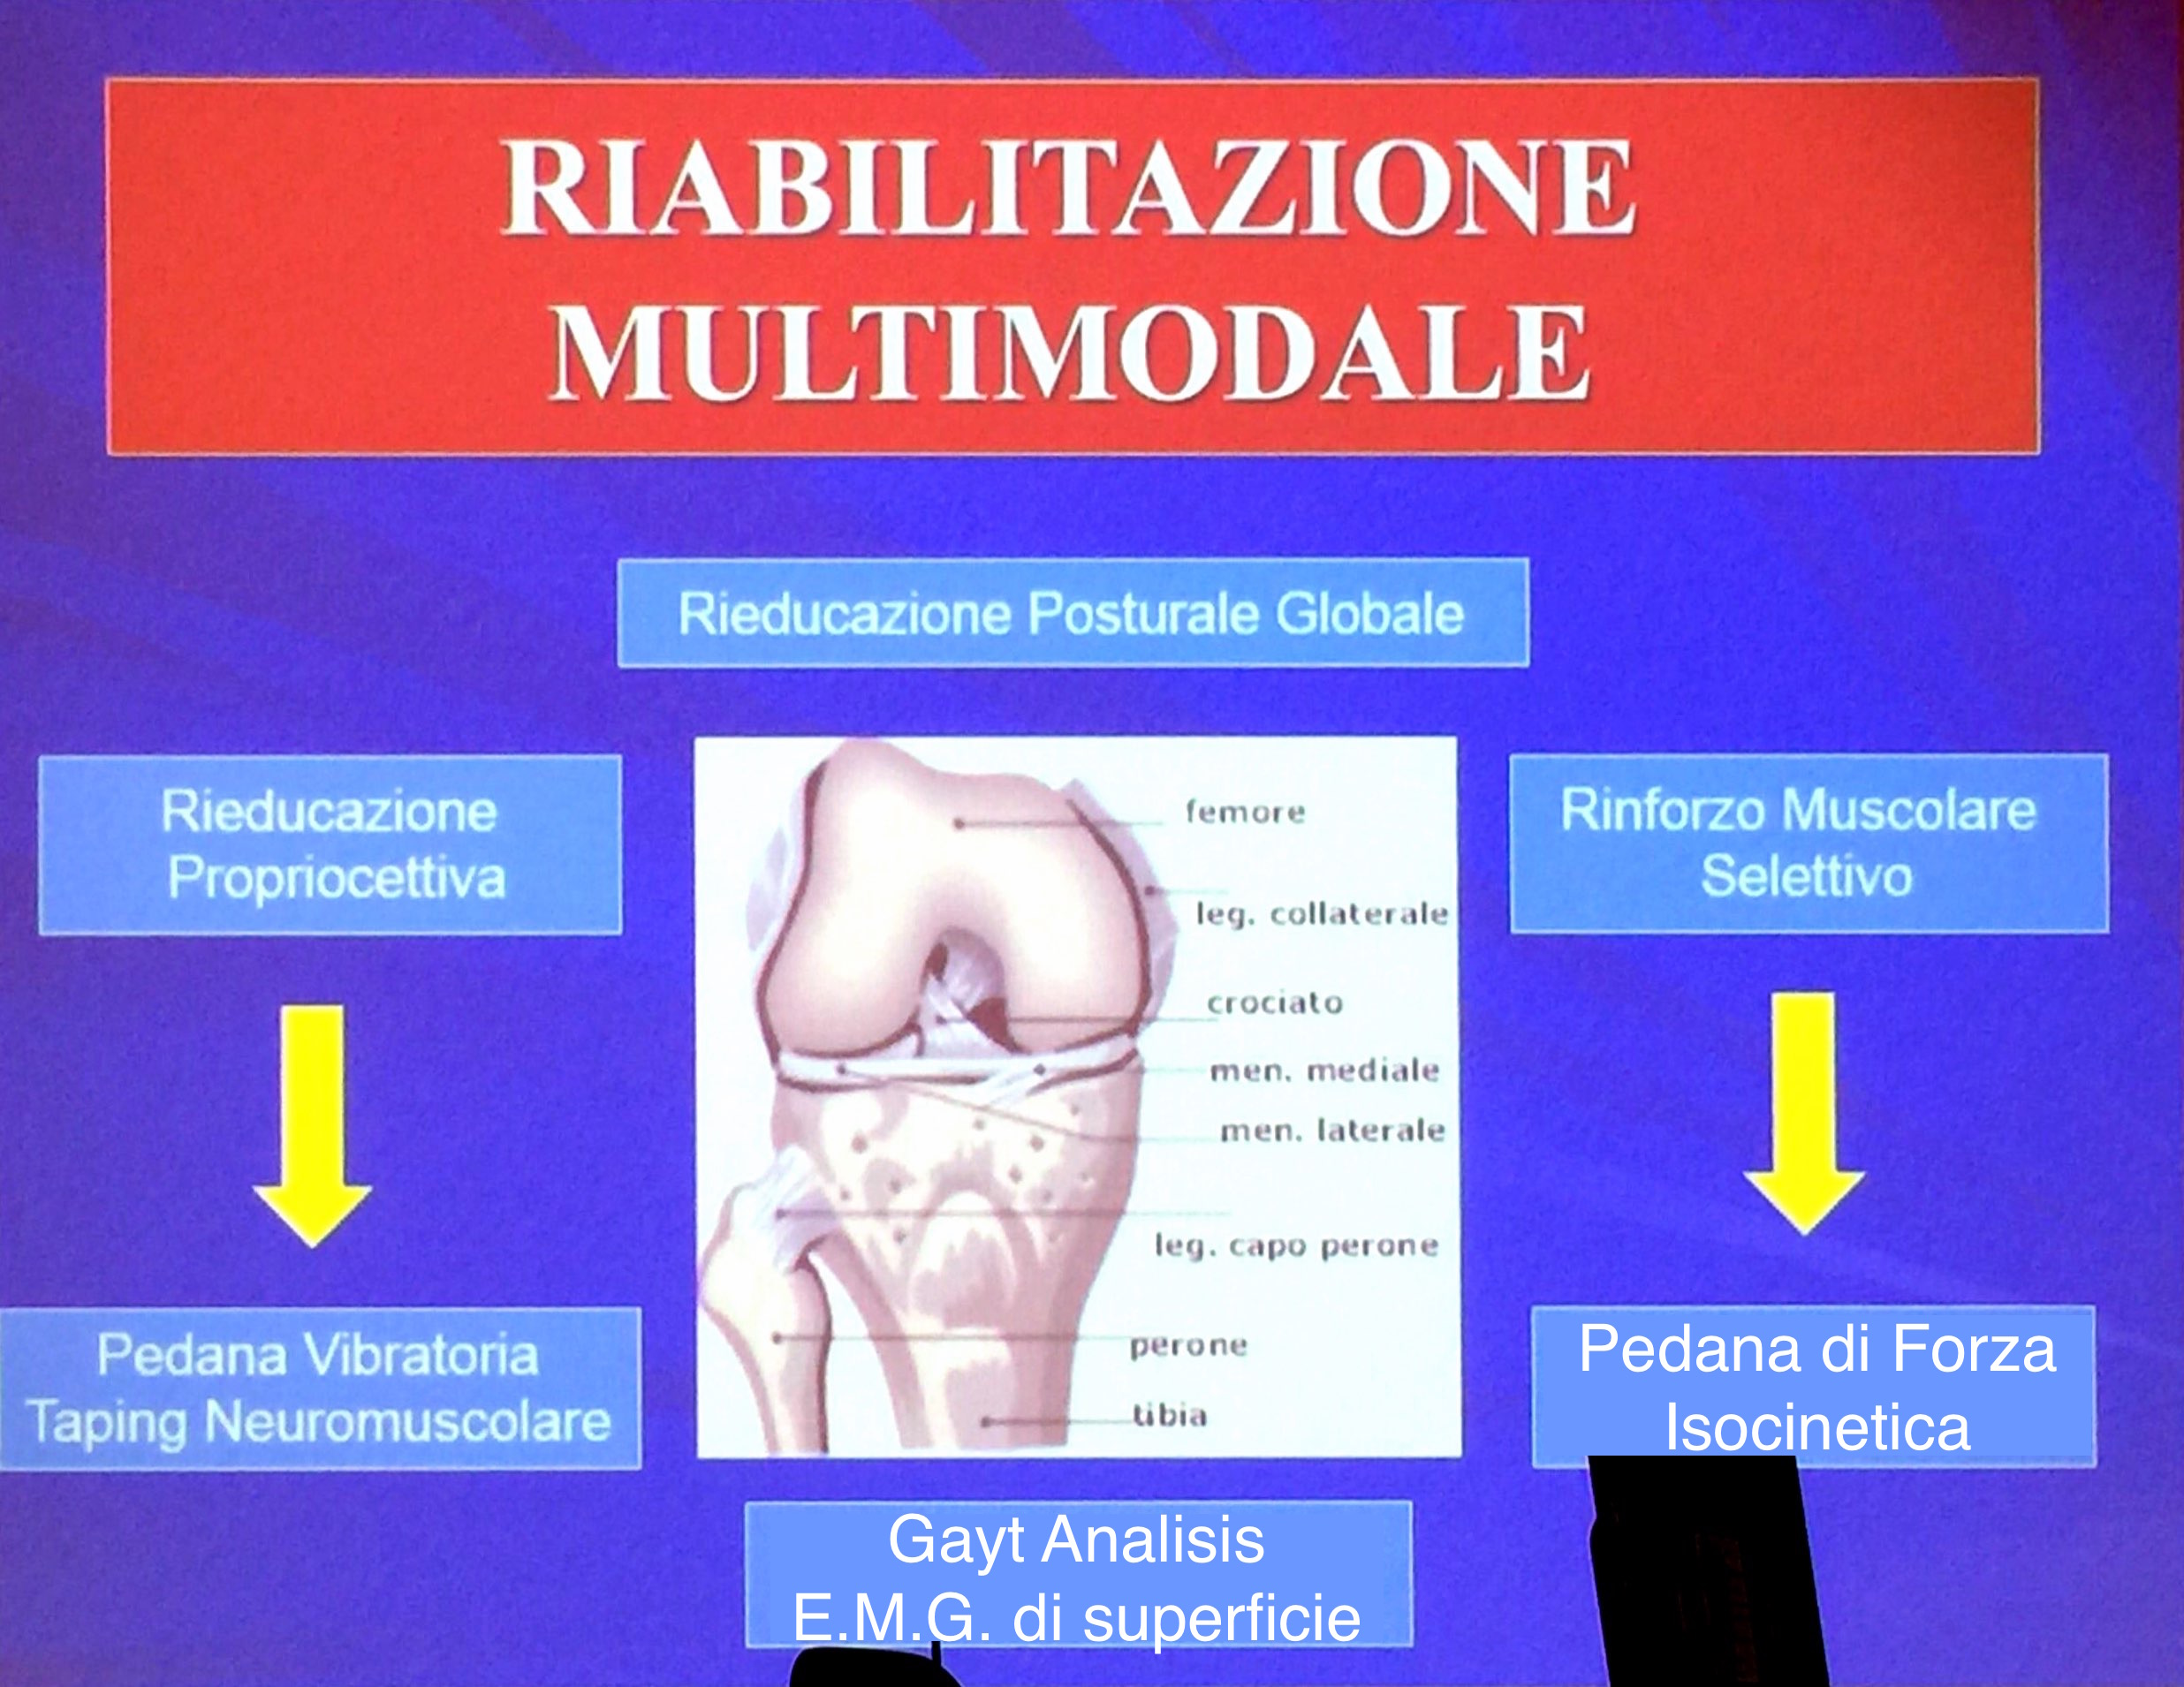
\includegraphics[width=0.00000in,height=0.00000in]{media/image19.jpeg}
ad esso viene applicato uno strumento che va in vibrazione (al posto
della vibrazione può essere applicato un tape e successivamente vengono
fatti fare degli esercizi con un manubrio). Si prende un dinamometro
meccanico che consente di valutare la forza di presa e di pinza della
mano del soggetto. Si misura la forza del soggetto prima del trattamento
con la vibrazione (o del trattamento con il tape) e si misura nuovamente
la forza dopo il trattamento con una serie di applicazioni di vibrazione
di poco tempo (o dopo aver eseguito una serie di esercizi con un
manubrio nel caso venissero applicati i tape). Ciò che è stato visto è
che dopo la stimolazione vibratoria (o dopo la serie di esercizi con il
tape) \emph{la forza del soggetto aumentava}. Questo è dovuto al fatto
che le vibrazioni (o il tape) fanno percepire un peso diverso,
\emph{minore}, per il muscolo e per l'articolazione.

NOTA BENE: Accenni alla nuova tecnologia*

\emph{*Il professore, QUEST'ANNO, ha deciso di non parlare delle nuove
tecnologie applicabili in questo campo e sottolinea il fatto che
verranno trattate l'anno prossimo a lezione in quanto i sistemi
descritti sopra diventeranno ``\emph{vecchi e desueti''}: non verranno
più utilizzate, ad esempio, le pedane di forza e per fare l'analisi del
movimento verranno utilizzati altri sistemi come gli
\textbf{accelerometri}.}

Gli \textbf{accelerometri} consentono di valutare:

\begin{enumerate}
\def\labelenumi{\arabic{enumi}.}
\item
  le \emph{componenti della forza} (come ad esempio le componenti
  angolari);

  il \emph{cammino} (con un solo accelerometro posizionato sotto il
  mento è possibile vedere come si muove il soggetto, come è il passo,
  il doppio appoggio, l'equilibrio, l'emipasso destro, l'emipasso
  sinistro).
\end{enumerate}

Tutti i dati ricavati sono dati strumentali, oggettivi.

\end{document}
